\chapter{Stand der Technik}
\section{Getränkemischmaschine}
\section{Hardware}
\section{Sprachverarbeitung}
\subsection{Spracherkennung}
\subsection{Vergleich verschiedener Ansätze}
Derzeit gibt es vier Hauptansätze für die Erstellung eines Chatbots:

- Musterabgleich - Musterabgleich und Antwortvorlagen (vorgefertigte Antworten)

- Grounding - logische Wissensgraphen und das Ziehen von Schlussfolgerungen aus diesen basierend auf diesen Graphen

- Suche - Abrufen von Text

- Generierungsmethoden - Statistik und maschinelles Lernen.

Die vier grundlegenden Ansätze zur Erstellung von Chatbots lassen sich kombiniert werden, was zu benutzerfreundlichen Chatbots führt. Viele Vielzahl von Anwendungen nutzen alle vier grundlegenden Methoden. Hybride Chatbots unterscheiden sich hauptsächlich darin, wie genau sie diese Ansätze kombinieren und wie viel Gewicht auf jeden einzelnen Ansatz gelegt wird.
\subsubsection{Musterabgleich}
Bei den ersten Chatbots basierte die Antwort auf die Nachricht eines Benutzers auf einem Mustervergleich. Diese Chatbots suchen nach Mustern im eingehenden Text und geben eine feste (gemusterte) Antwort, wenn eine Übereinstimmung gefunden wird (//BUCH).
Solche rudimentären Dialogsysteme sind vor allem in automatisierten Benutzerunterstützungssystemen mit interaktiven Sprachmenüs nützlich, wo es möglich ist, das Gespräch an einen Menschen weiterzuleiten, wenn der Chatbot keine Antwortmuster mehr hat.
Da es viele NLP-Dienstprogramme in Python-Paketen gibt, ist es möglich, komplexere Chatbots auf der Grundlage von Mustervergleichen zu erstellen, indem man die Bot-Logik nach und nach direkt in Python mit regulären Ausdrücken und Suchmustern aufbaut.
1995 machte sich Richard Wallace daran, einen allgemeinen Rahmen für die Erstellung von Chatbots auf der Grundlage des Pattern-Matching-Ansatzes zu schaffen. Zwischen 1995 und 2002 schuf seine Entwicklergemeinschaft die Artificial Intelligence Markup Language (AIML) zur Beschreibung von Mustern und Chatbot-Antworten.
AIML ist eine deklarative Sprache, die auf dem XML-Standard basiert, der die Sprachkonstrukte und Datenstrukturen einschränkt, die im Bot verwendet werden dürfen. Ein Chatbot, der auf AIML basiert, sieht folgendermaßen aus:
\begin{figure}[H]
    \centering
    \fbox{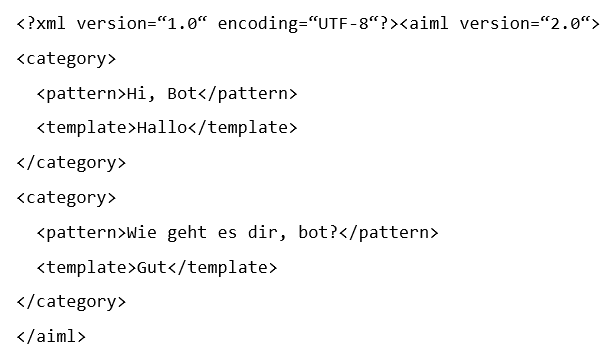
\includegraphics[width=0.8\textwidth]{Bilder_Kapitel_2/aiml_bot.png}}
    \caption{\label{figure:Aiml_Bot}AIML Chatbot}
\end{figure}
\noindent
Eine der Einschränkungen von AIML ist die Art der Muster, die abgeglichen werden können und auf die reagiert wird. Der AIML-Kern (Pattern Matching Engine) reagiert nur auf Eingabetext, der einem vom Entwickler manuell vorgegebenen Muster entspricht. Unscharfe Suchanfragen, Smileys, Satzzeichen, Tippfehler oder falsch geschriebene Wörter sind nicht erlaubt, es findet kein automatischer Abgleich statt. In AIML müssen alle Synonyme manuell einzeln beschrieben werden.
\subsubsection{Grounding}
\subsubsection{Suche}
\subsubsection{Generierungsmethoden}
\endinput